\section{What is planning? Why is it important? What happens if it is not done correctly?}
\begin{itemize}
    \item Planning: process of analyzing, evaluate, decide and organize activities in advance.
    \item Three fundamental steps: define the goal, evaluate options, choose and confirm the best option to achieve the goal.
    \item Planning is on 2 levels: strategic and tactical.
    \item Failing to plan properly can end in terrible results.
\end{itemize}

%%%%%%%%%%%%%%%%%%%%%%%%%%%%%%%%%%%%%%%%%%%%%%%%%%%%%%
\section{Why is planning so critical in PM?}
\begin{itemize}
    \item Planning is the fundamental work of the project manager.
    \item It is when the PM demontrates their expertise.
    \item You cand devide planning in 2:
        \begin{itemize}
            \item Things the PM does not know.
            \item Things the PM does know and can't control. Here risk assesment, estimations and forecasts need to be covered, this is done using planning.
        \end{itemize}
    
    \item Good planning gives great results: optimize work, ensures same expectations, avoids costly errors. The better planning the more chances of success the project has.
    \item People also work much better with direction, when they understand what to do, how to do it and when they must do it.
    \item Planning is your strategy to succeed. Despite this planning is often criminally underestimated. People think that the sooner they execute (without planning) they better but in reality the more effort is expended in the planning phase the less effort is needed in during the execution phase. This is the 80/20 rule. More planning means less replanning and delays during execution.
\end{itemize}

%%%%%%%%%%%%%%%%%%%%%%%%%%%%%%%%%%%%%%%%%%%%%%%%%%%%%%
\section{What is the cost of change in projects?}
\begin{itemize}
    \item Each change to the original project outlined in the project charter impacts cost and time, often both. The aditional budget, time, resources, and coordination efforts are the ''cost´´.
    \item Remember the triangle of contraints:
        \begin{figure}[H]
            \centering
            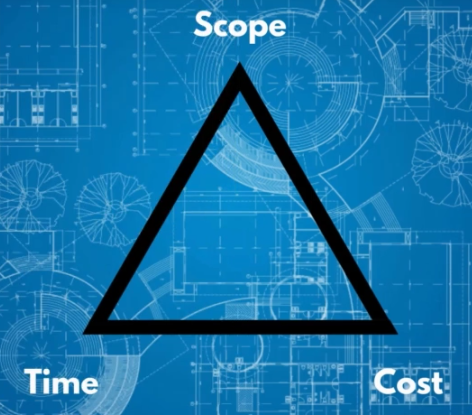
\includegraphics[width=\width\textwidth]{./figs/20221021152932.png}
            %\caption{}
        \end{figure}
    
    \item When the change is made also impacts, since it is cheaper if the change is thought out during the initial phase of the project than if the project is near the end.
    \item The more time passes during execution of the project the higher cost of change it has:
        \begin{figure}[H]
            \centering
            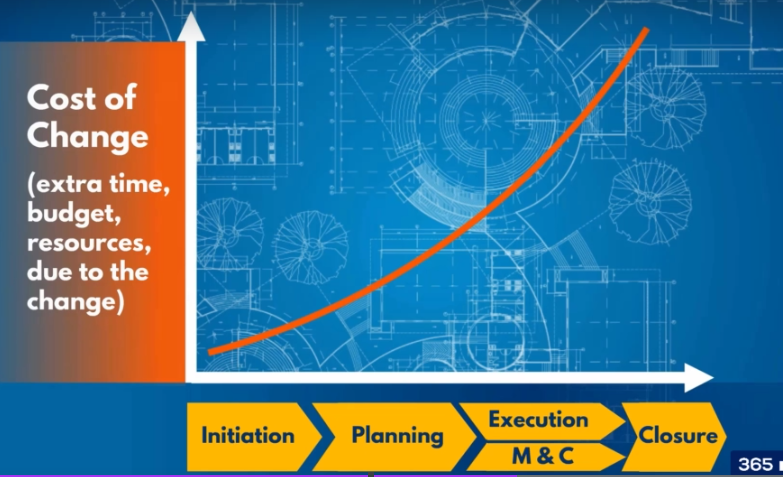
\includegraphics[width=\width\textwidth]{./figs/20221021153117.png}
            %\caption{}
        \end{figure}
    
    \item A PM must take into account potential changes the project might need in advance and that is why they need to be master planners.
\end{itemize}

%%%%%%%%%%%%%%%%%%%%%%%%%%%%%%%%%%%%%%%%%%%%%%%%%%%%%%
\section{What to do before you start?}
\begin{itemize}
    \item There are some considerations the PM needs to take into account during planning:
        \begin{enumerate}
            \item The PM must asses their own knowledge of the required work. (Is it enough to plan?)
            \item The PM must know all the project stakeholders.
            \item The PM must recall lessons learned. (Has this project been done before? If so what lessons can we get from the previous projects?)
            \item What about knowledge gaps? (a good project manager is not someone who knows everything, but someone who can identify their own shortcomings and find the right people to compensate for them.)
        \end{enumerate}
    
    \item A PM must determine how much time they need to put all the pieces of a project together. Also decide with who they will keep in contact with. And also reafirm the expectations to stakeholders.
    \item In meetings with stakeholders they must prepare with an agenda, a goal, and a comprehensive list of topics to cover.
    \item PM need to plan for everything.
\end{itemize}

%%%%%%%%%%%%%%%%%%%%%%%%%%%%%%%%%%%%%%%%%%%%%%%%%%%%%%
\section{Project management insights}
\begin{itemize}
    \item Changes are frequent during planning.
        \begin{itemize}
            \item New information can arise at any time.
        \end{itemize}
    
    \item Planning simple tasks:
        \begin{itemize}
            \item A simple task must be planned too. 
            \item A meeting needs to be planned out by determining the participants, day time, room for the meeting, flipchart, and sending out the invitations.
        \end{itemize}
    
    \item Tasks with unplanned time durations:
        \begin{itemize}
            \item Some tasks you cannot estimate, especially if they depend on other people to come to fruition. These tasks can become problematic and can delay the project if not managed correctly.
            \item Example of hiring an engineer, you write to HR, after a day they respond they need more details, you reach out to IT in order to get the details, 2 days pass and you have the details, but the details need to be verified by the head of IT that is in vacations and thus what could have easily been planned to take 2 days become 8+ days.
        \end{itemize}
\end{itemize}

%%%%%%%%%%%%%%%%%%%%%%%%%%%%%%%%%%%%%%%%%%%%%%%%%%%%%%ss
\section{Scope planning}
\begin{itemize}
    \item At this stage the PM should have information enough to start planning. The planning has its own structure.
    \item The first thing a PM needs to do is to define the project scope.
\end{itemize}

\subsection{Setting up a scope}
\begin{itemize}
    \item Establish the questions that need to be answered.
    \item In the lamborarri showroom example we need to define how many floors will it have, who will be in charge of what, etcetera.
    \item Remember scope means what exactly does the project team need to do.
        \begin{figure}[H]
            \centering
            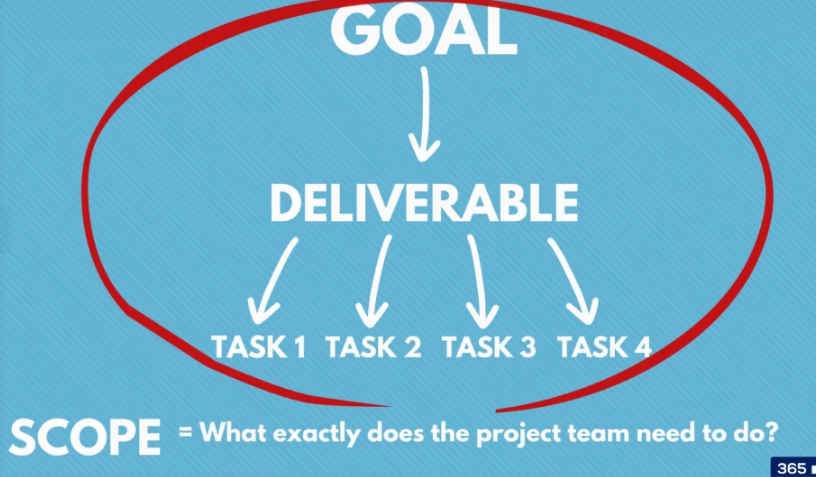
\includegraphics[width=\width\textwidth]{./figs/20221021155322.png}
            %\caption{}
        \end{figure}
    
    \item Once the goal has been established we can then define deliverables.
        \begin{itemize}
            \item A deliverable must have all the requirements clearly established. 
            \item An example of deliverables is the following:
                \begin{figure}[H]
                    \centering
                    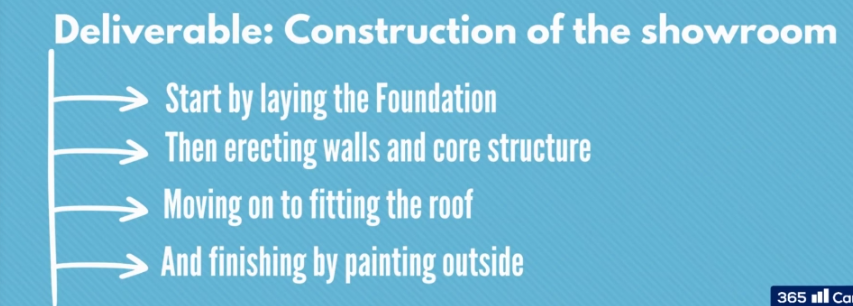
\includegraphics[width=\width\textwidth]{./figs/20221021160849.png}
                    %\caption{}
                \end{figure}
        \end{itemize}
    
    \item For example lets say that in the land in which we plan to build the show room there is already a building, we need to factor this into our scope since we cannot do anything related to the actual project until we demolish the building.
    \item Product scope: the tasks that need to be done to produce the product.
    \item Project scope: all that you need to do in order to achieve the project goal. This includes the product scope.
    \item A scope needs to be described in detail, a scope definition needs to include what is not in the scope also. 
    \item Take into account that we are not looking for cent precision in planning, if you forgot some trivial thing then that can be added later on with no major incident but if you forgot something big such as a million dollars worth of details then that will be a problem.
    \item In the showroom project this needs to be agreed between the construction company and the city.
\end{itemize}

\subsection{Scope steps}
\begin{itemize}
    \item Assesing information on the project scope.
    \item Gathering details on project requirement and expectation.
    \item Using expertise to cover grey areas.
    \item Documenting everything. (If something arises that need to be checked then it must be available.)
\end{itemize}

%%%%%%%%%%%%%%%%%%%%%%%%%%%%%%%%%%%%%%%%%%%%%%%%%%%%%%
\section{Scope part 2}
\begin{itemize}
    \item Recap:
        \begin{itemize}
            \item We analyze the available information.
            \item We gather detailed requirements and expectations.
            \item We document the scope.
        \end{itemize}

    \item Now for a low level look at scope planning:
        \begin{itemize}
            \item The PM analyses high-level information gained in the initiation stage from the project charter, discussions with the sponsor and clients, as well as stakeholders.
            \item Then gather detailed requirements and expectations, such as the sponsors and managers, the sponsor and senior manager are a reliable source of information on scope if the PM asks the right questions.
            \item The more information the PM gathers the better.
            \item Then with all this information the PM must document all this in a document called a scope statement document. This document is looked at as a sort of contract, between the PM and stakeholders, it outlines what the PM has commited and has not commited to do. 
        \end{itemize}
    
    \item The scope statement document is not user friendly. 
    \item This is why the scope statement needs to be reformated and split into deliverables and then each deliverable must be assigned to a specific person.
        \begin{figure}[H]
            \centering
            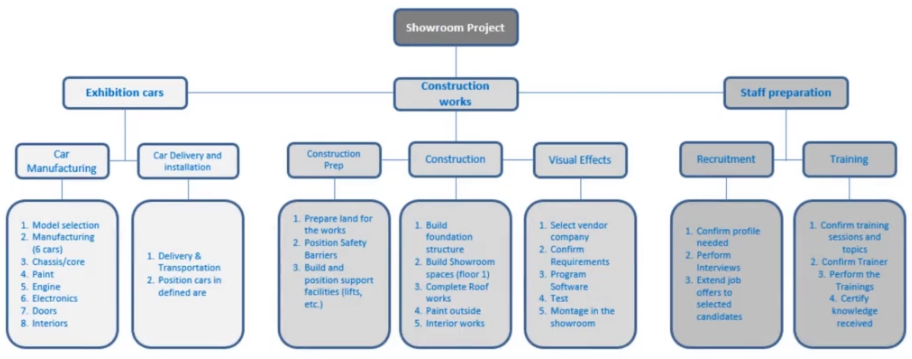
\includegraphics[width=\width\textwidth]{./figs/20221021162232.png}
            %\caption{}
        \end{figure}
    
    \item For an even more user-friendly experience the PM creates an activity list. Which details the task, person, activity, etcetera. This to make it absolutely clear what will be done, by who and by which date. This document can be refered to by anyone.
        \begin{figure}[H]
            \centering
            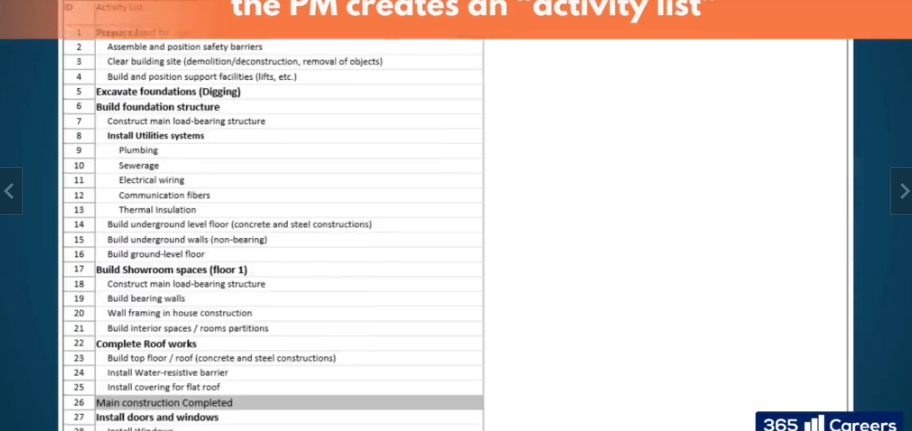
\includegraphics[width=\width\textwidth]{./figs/20221021162346.png}
            %\caption{}
        \end{figure}
    
    \item Note that there are three documents involved here that contain the same information in different formats:
        \begin{figure}[H]
            \centering
            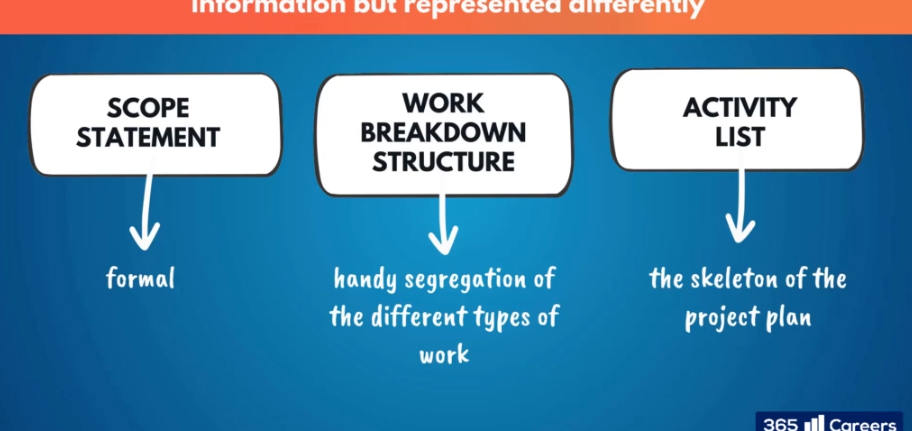
\includegraphics[width=\width\textwidth]{./figs/20221021162430.png}
            %\caption{}
        \end{figure}
\end{itemize}